\newpage
\subsection{Manufacturing Drawings and Sketches}
\label{sec:mech_drawings}
% \begin{figure}[h!] 
% 		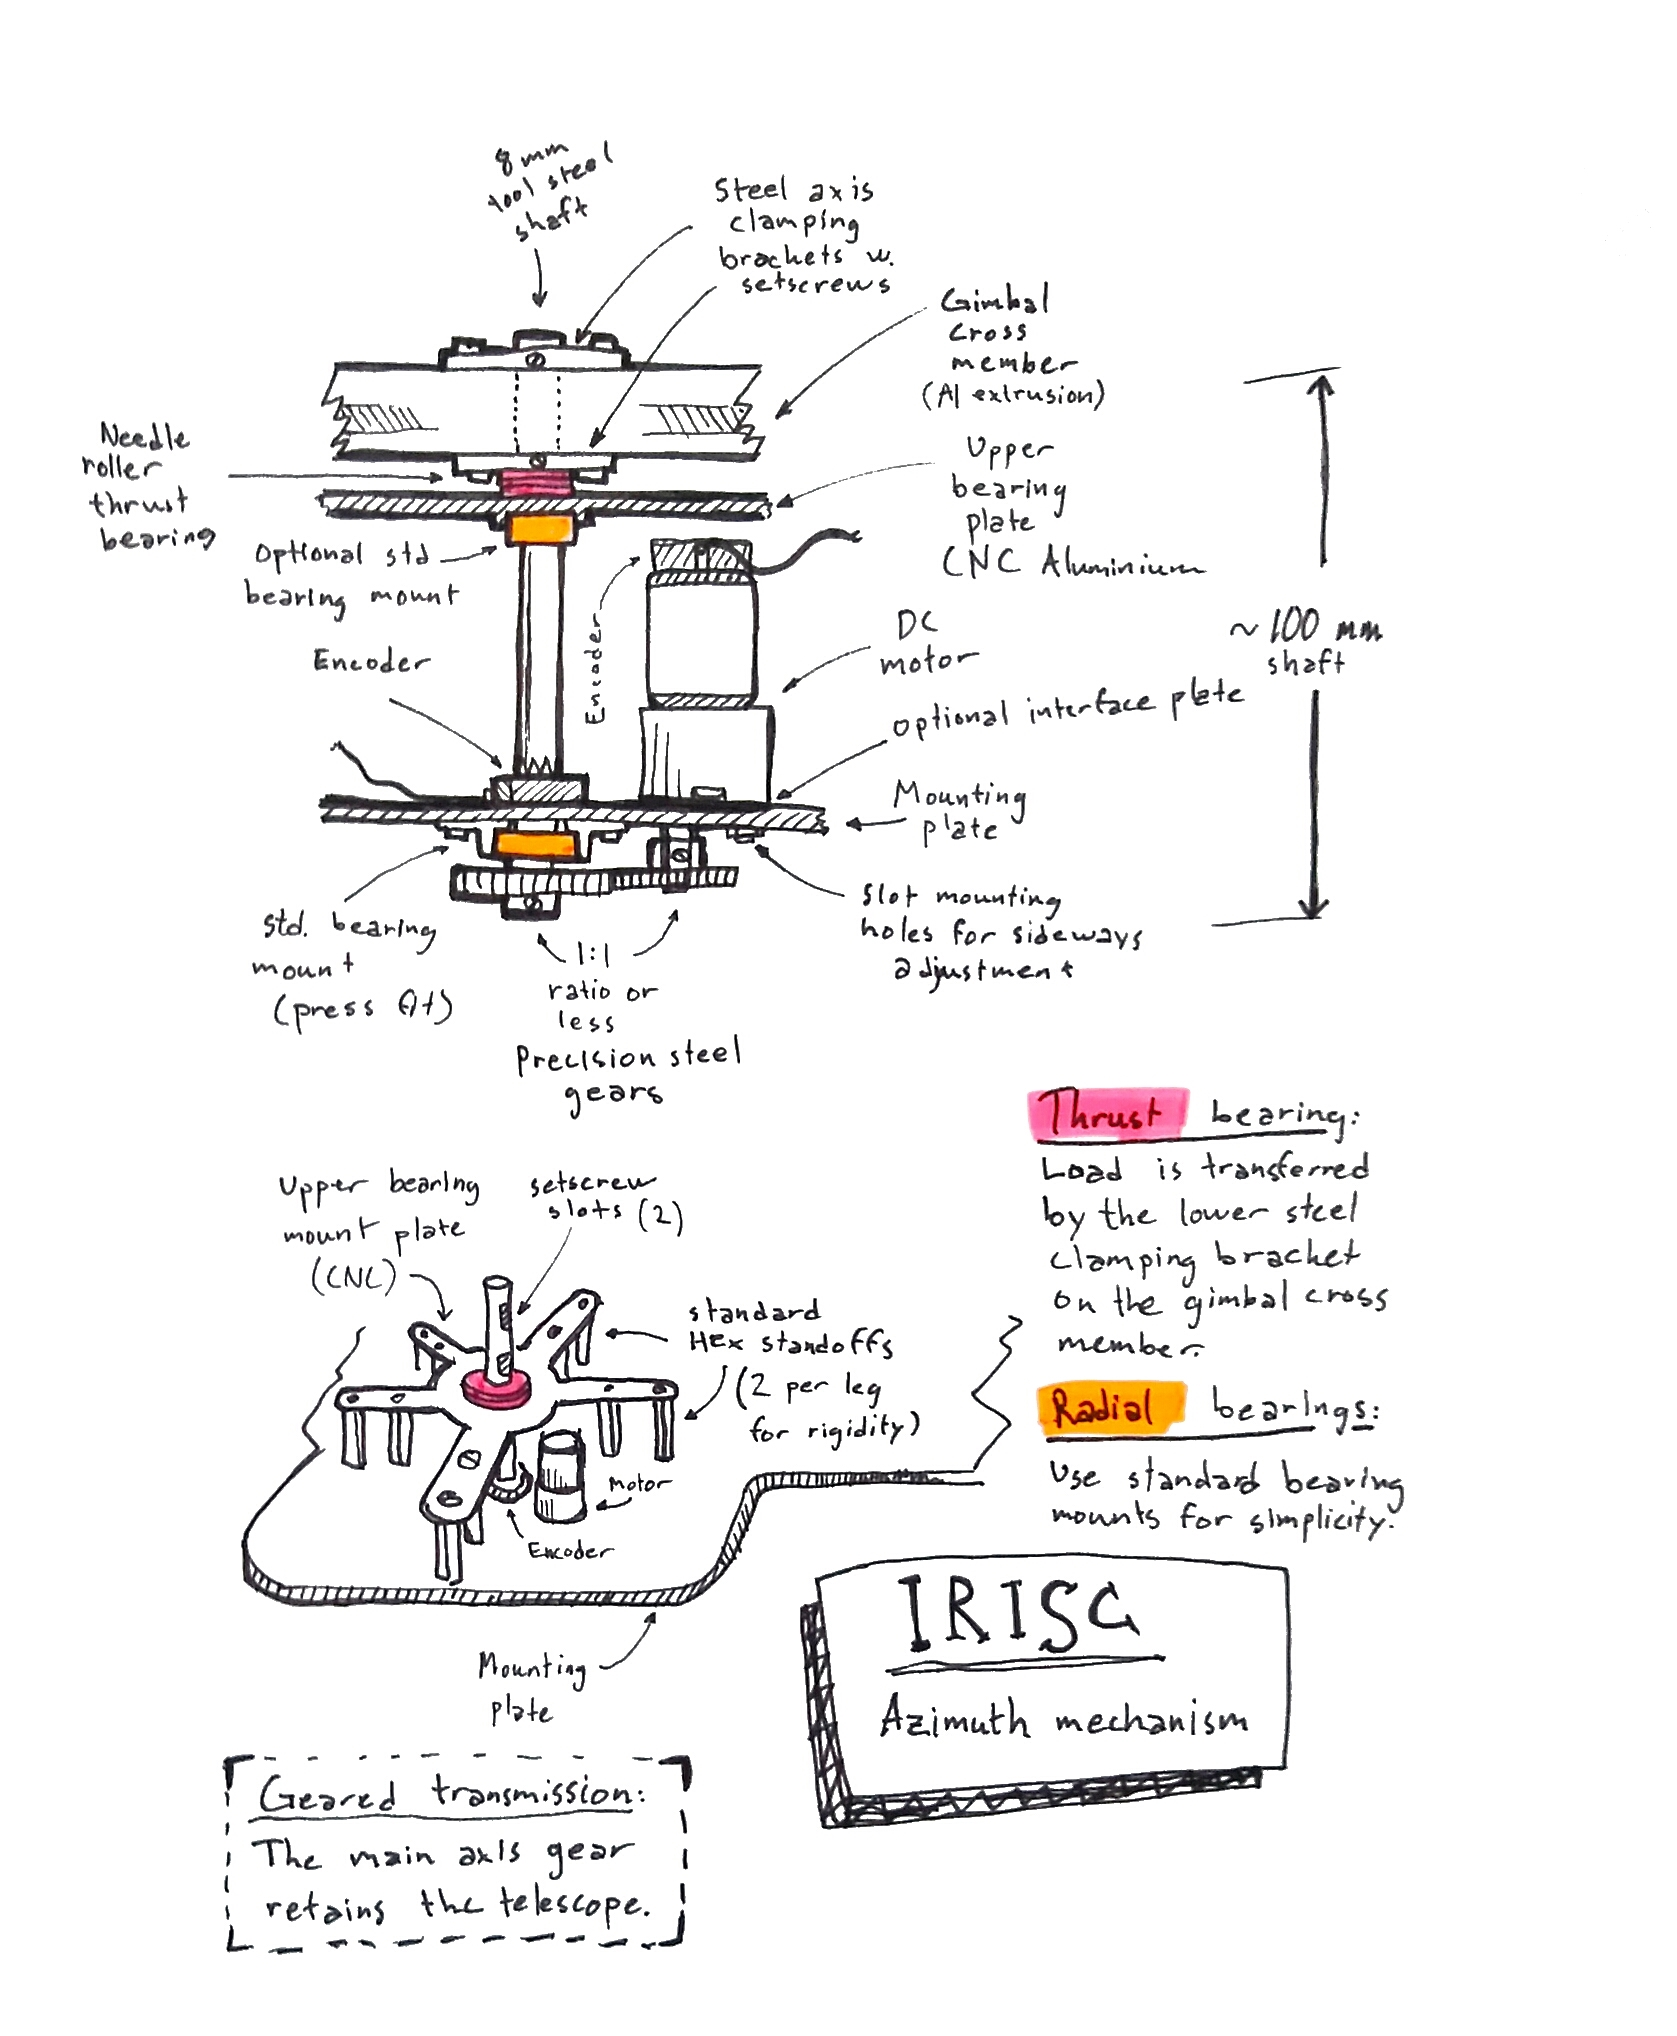
\includegraphics[width=\textwidth]{appendix/img/mechanical_sketches/azimuth_mechanism.jpg}
% 		\caption{Azimuth mechanism sketch.}
% 		\label{img:az_sketch}
% \end{figure}
% \newpage
% \begin{figure}[h!] 
% 		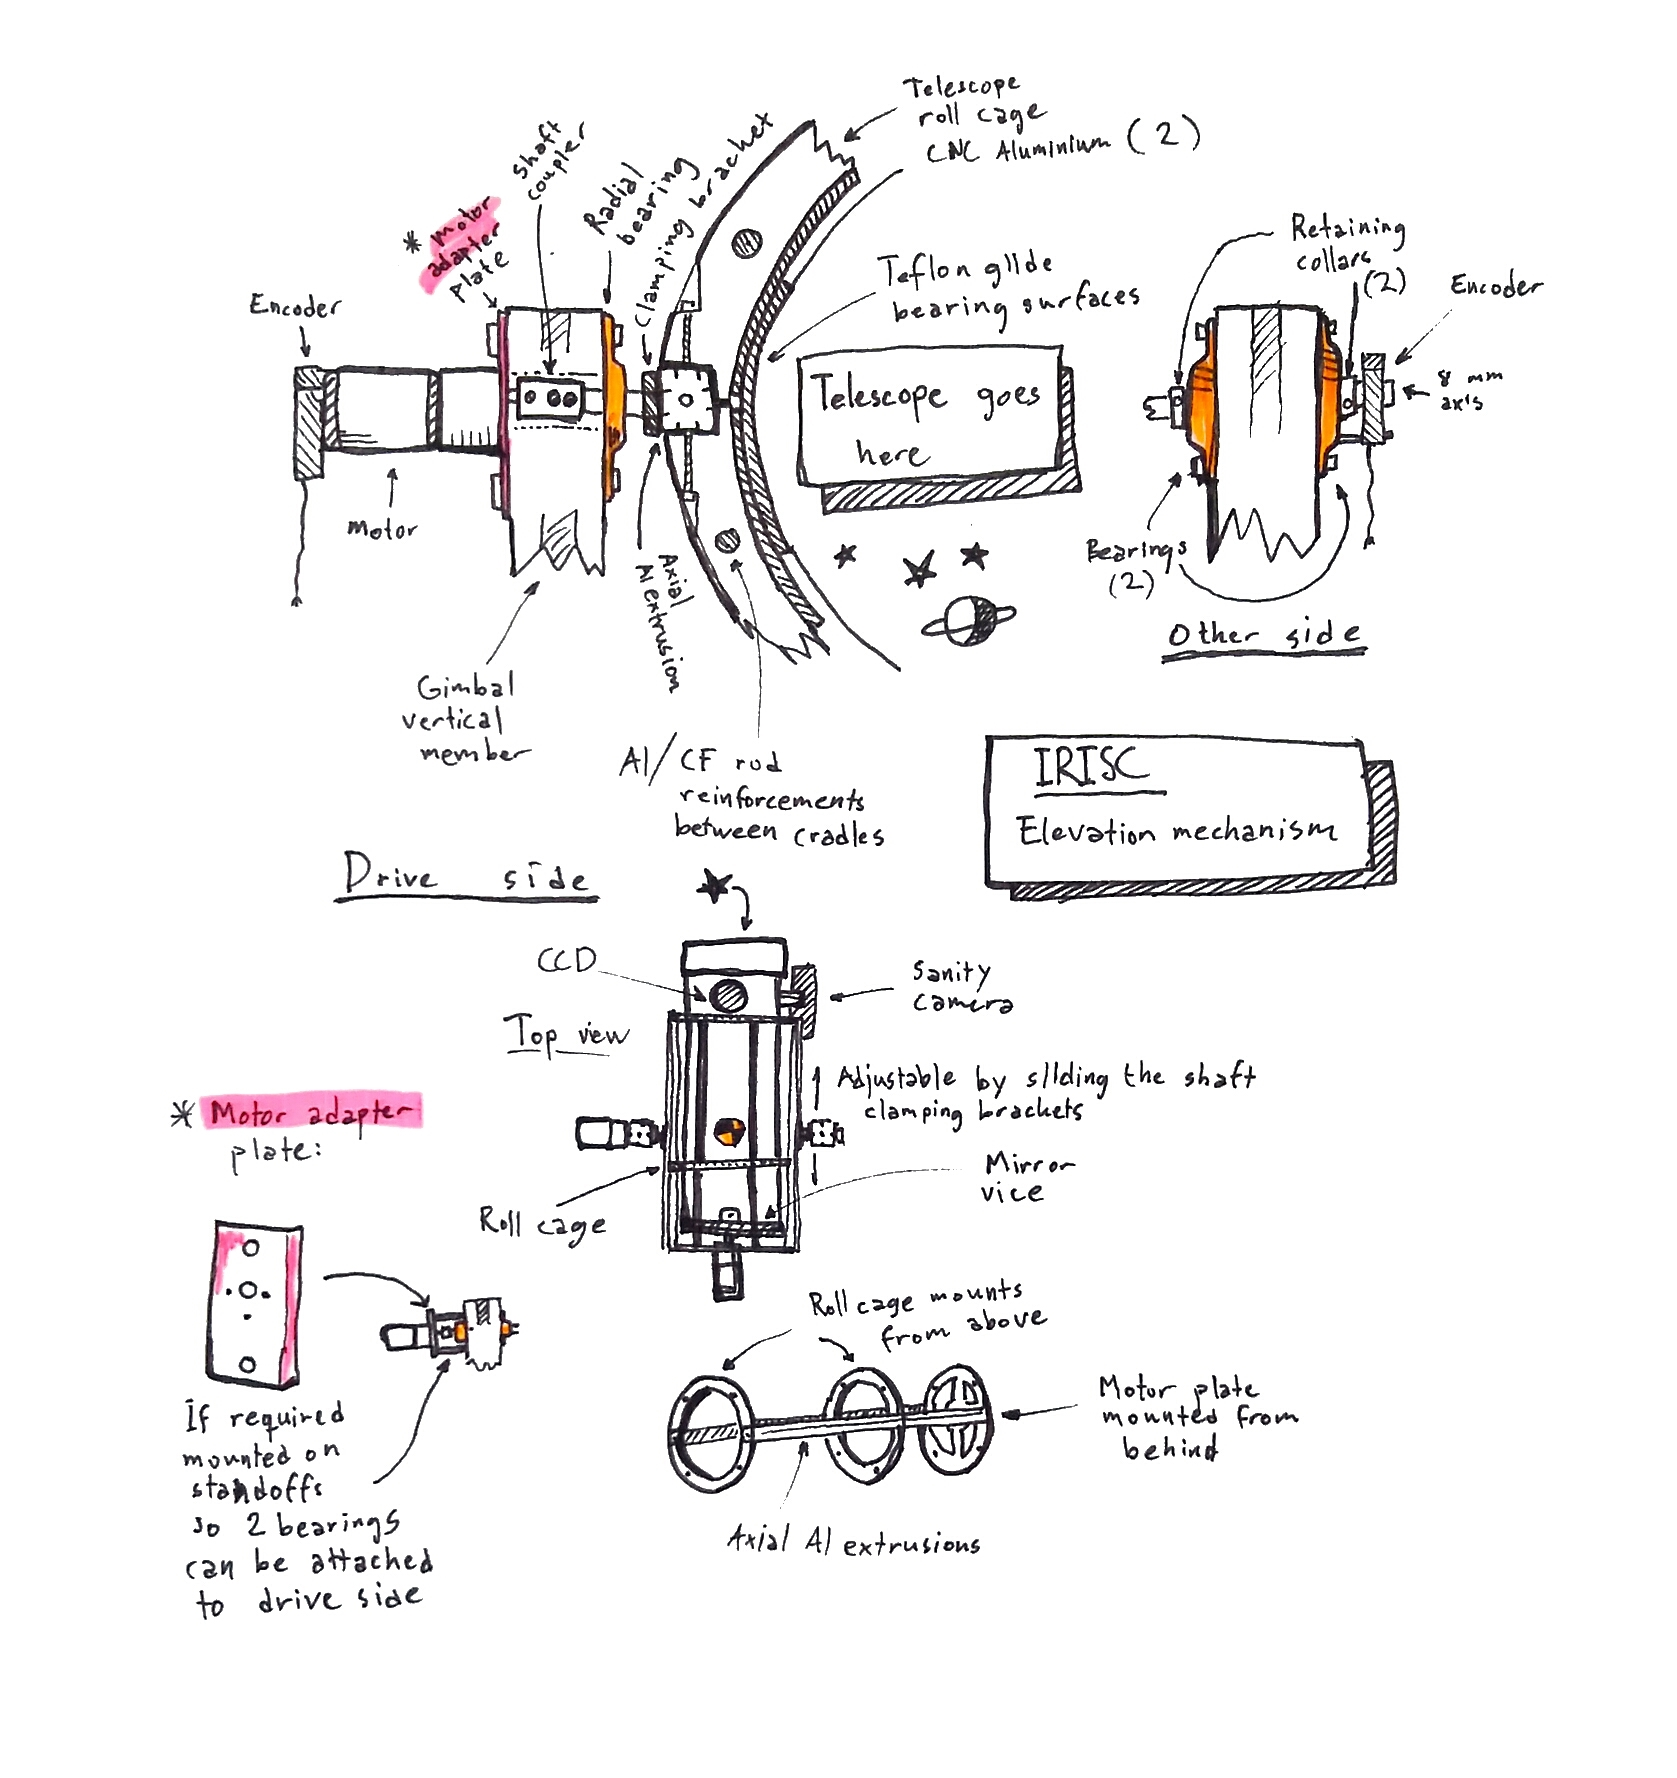
\includegraphics[width=\textwidth]{appendix/img/mechanical_sketches/elevation_mechanism.jpg}
% 		\caption{Elevation mechanism and roll cage sketch.}
% 		\label{img:el_sketch}
% \end{figure}
% \newpage
% \begin{figure}[h!] 
% 		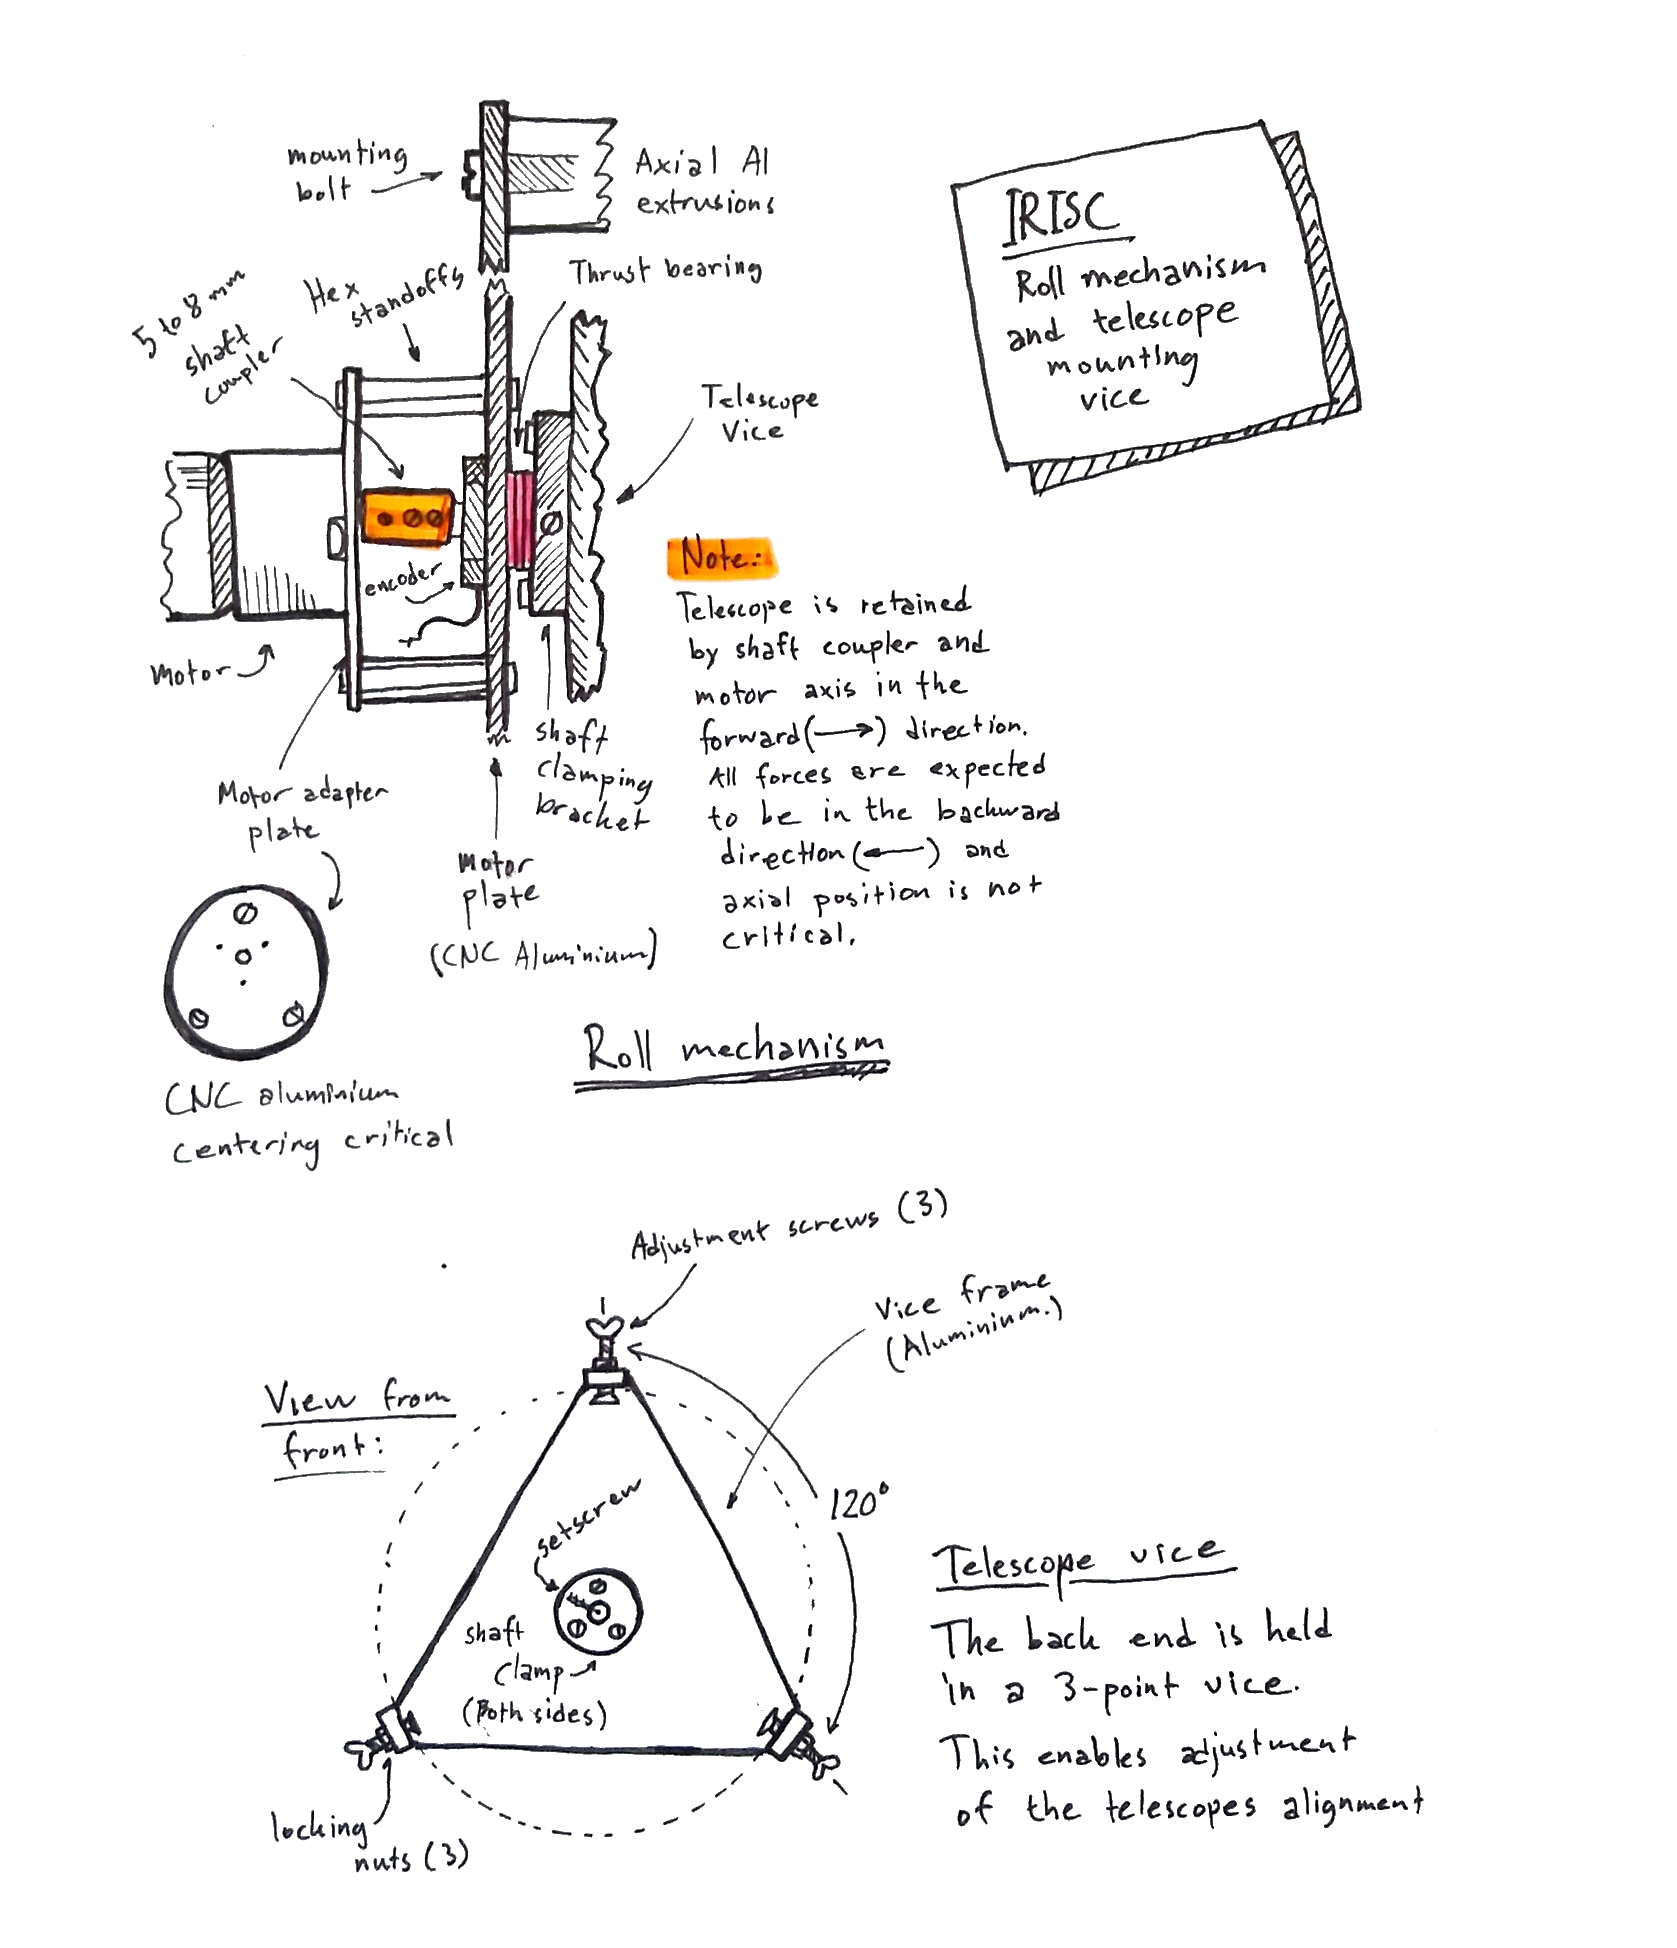
\includegraphics[width=\textwidth]{appendix/img/mechanical_sketches/roll_mechanism.jpg}
% 		\caption{Roll mechanism and telescope retaining vice sketch.}
% 		\label{img:roll_sketch}
% \end{figure}

\begin{figure}[H]
	\centering 
	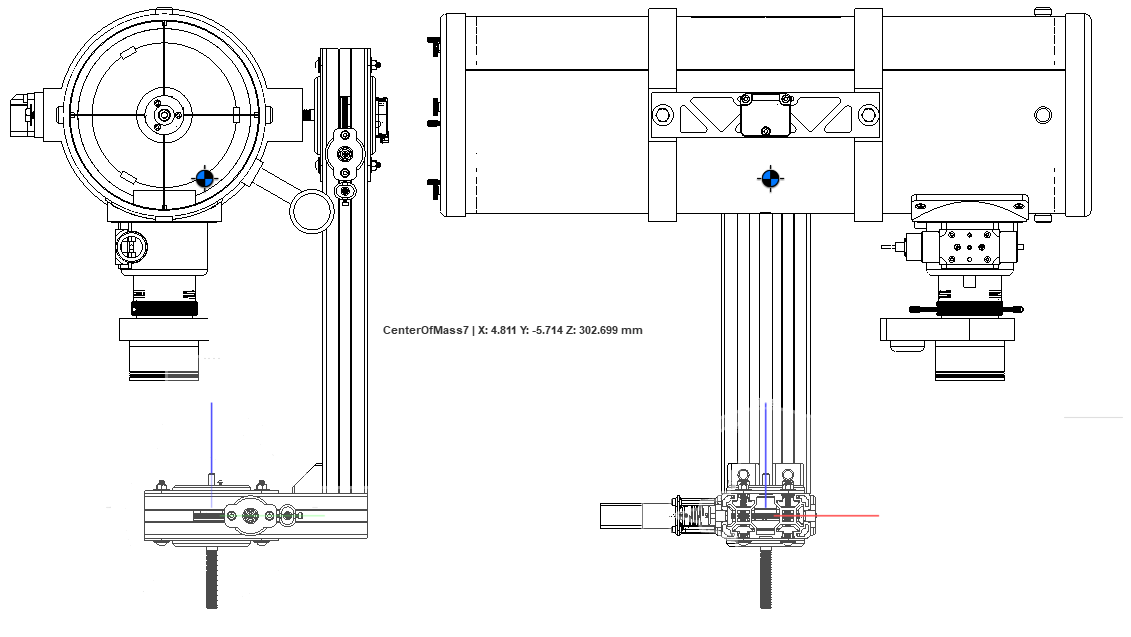
\includegraphics[scale=0.6]{4-experiment-design/img/mechanical/COM.png}
	\caption{Gimbal center of mass estimation.}
	\label{fig::mechanical::COM}
\end{figure}

\begin{landscape}
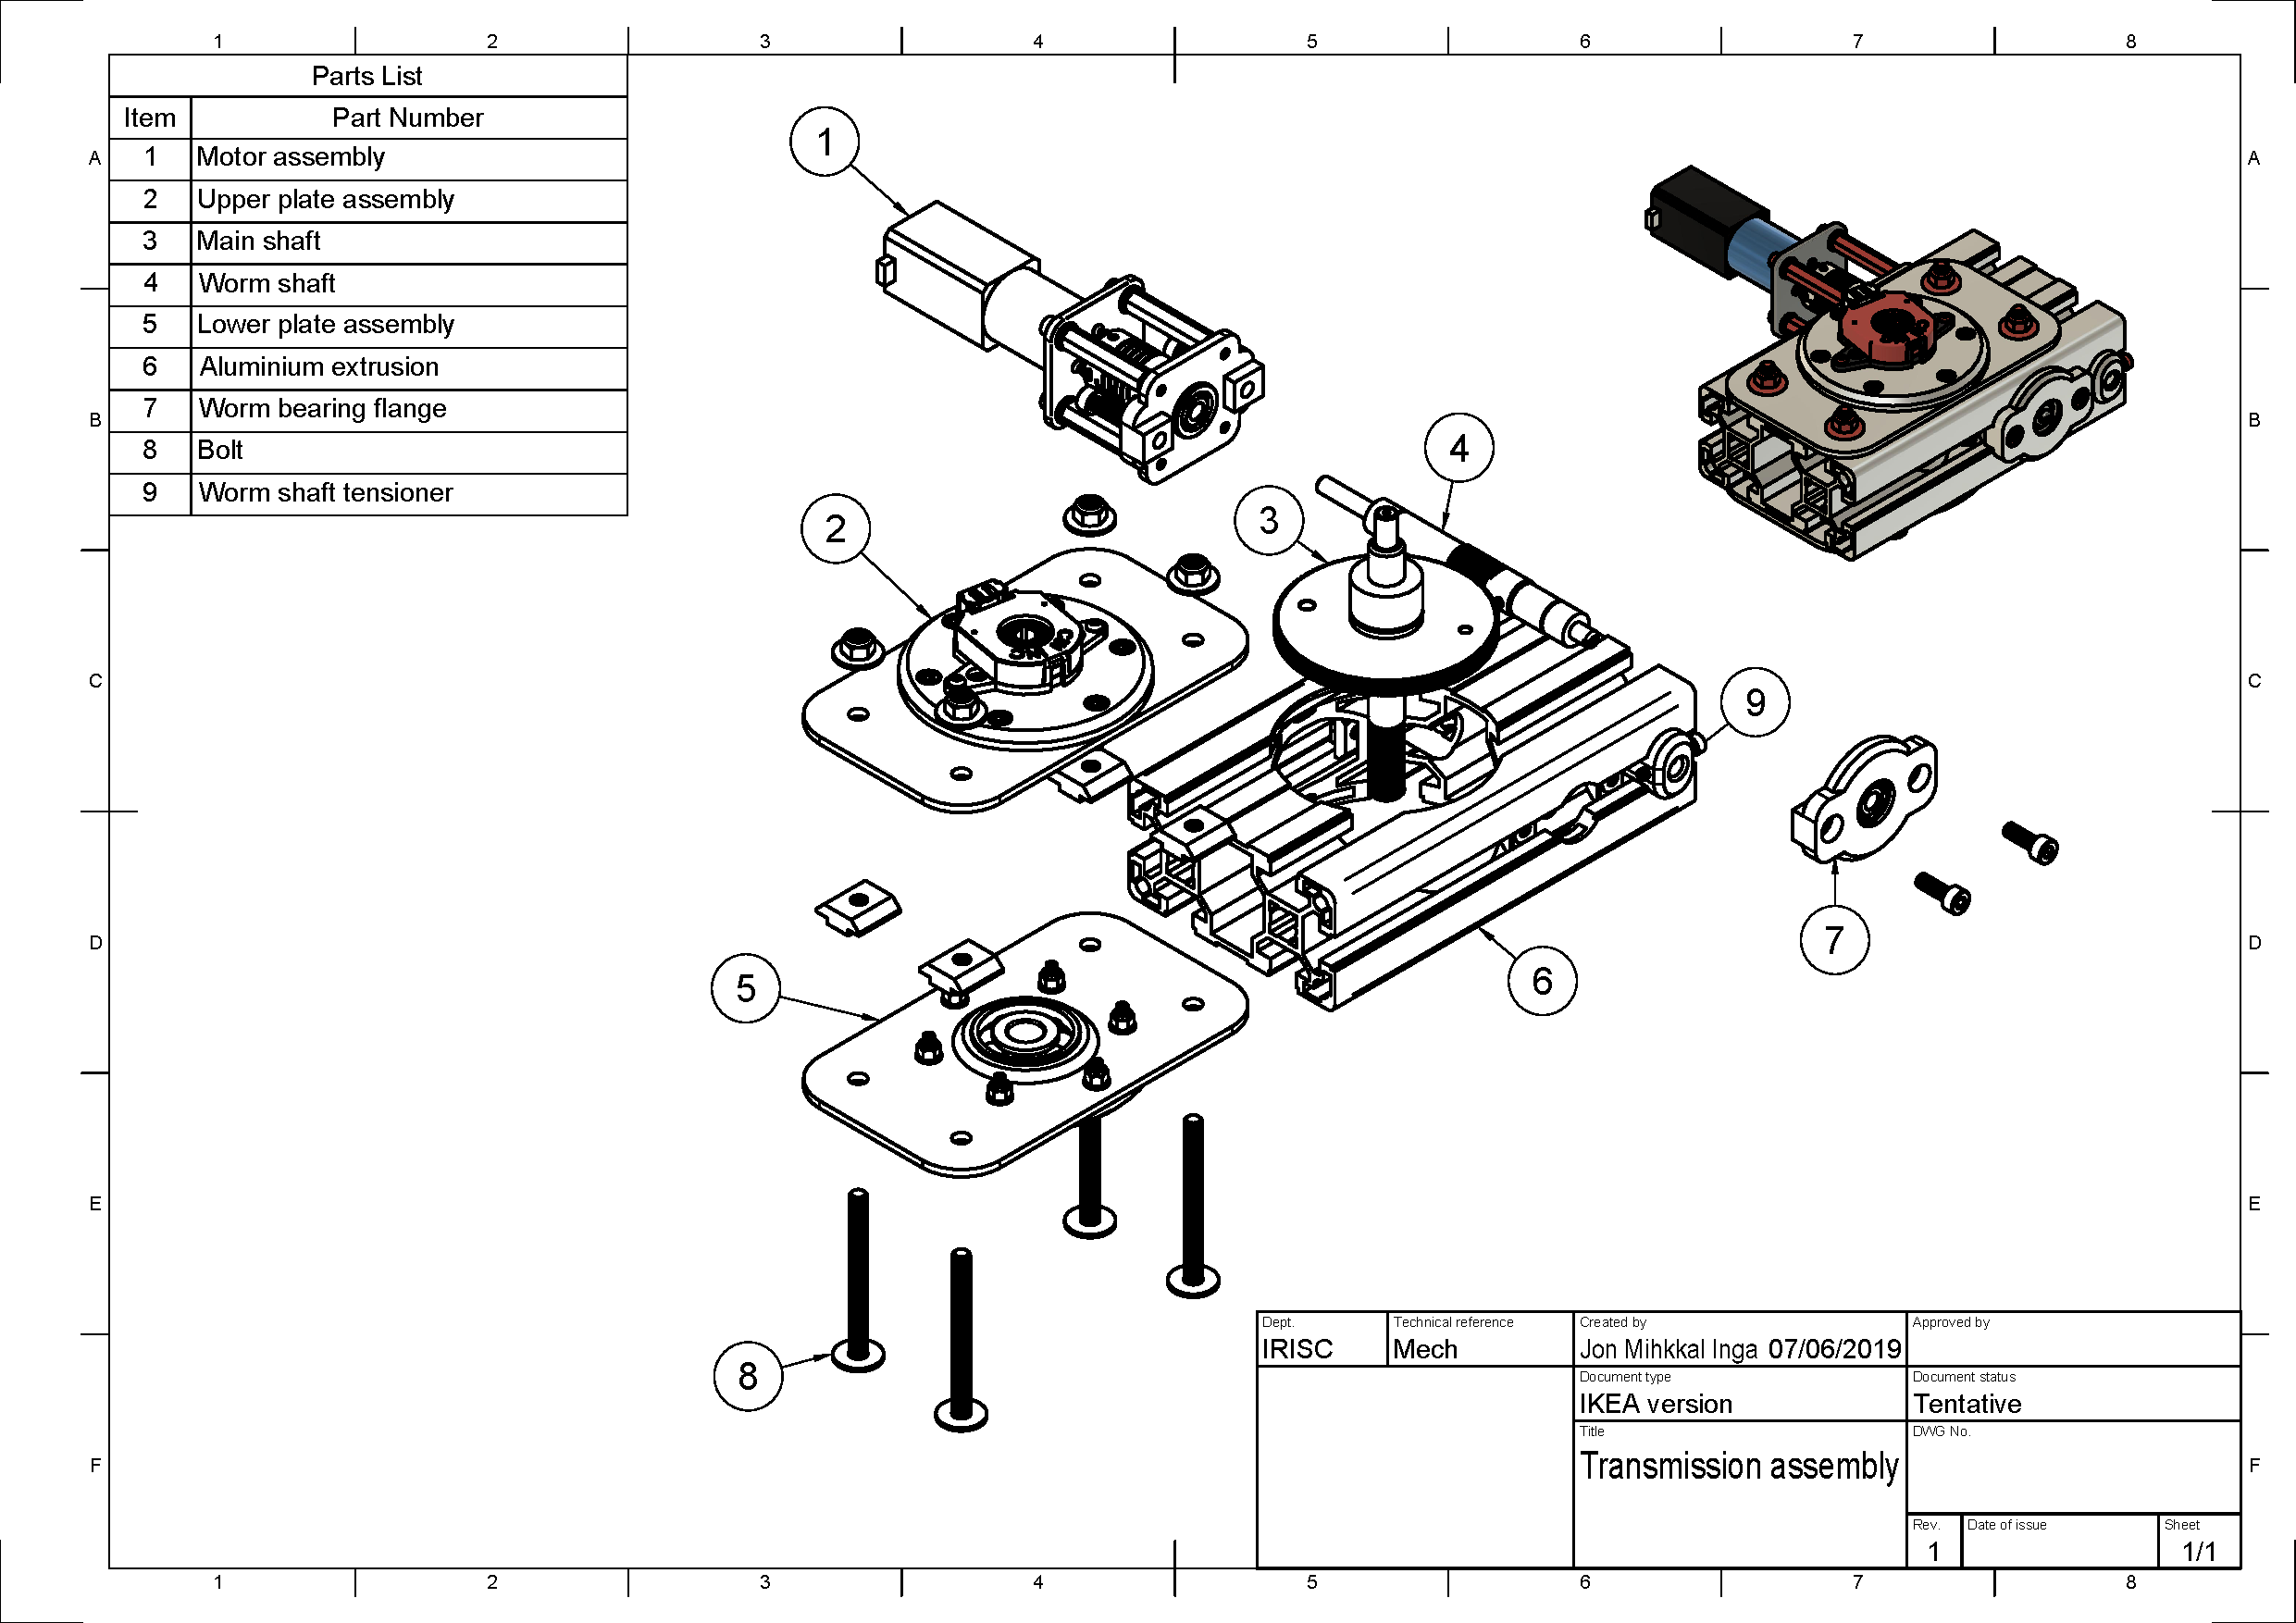
\includegraphics[scale=0.5]{appendix/img/mechanical_sketches/Transmission_Assembly.pdf}

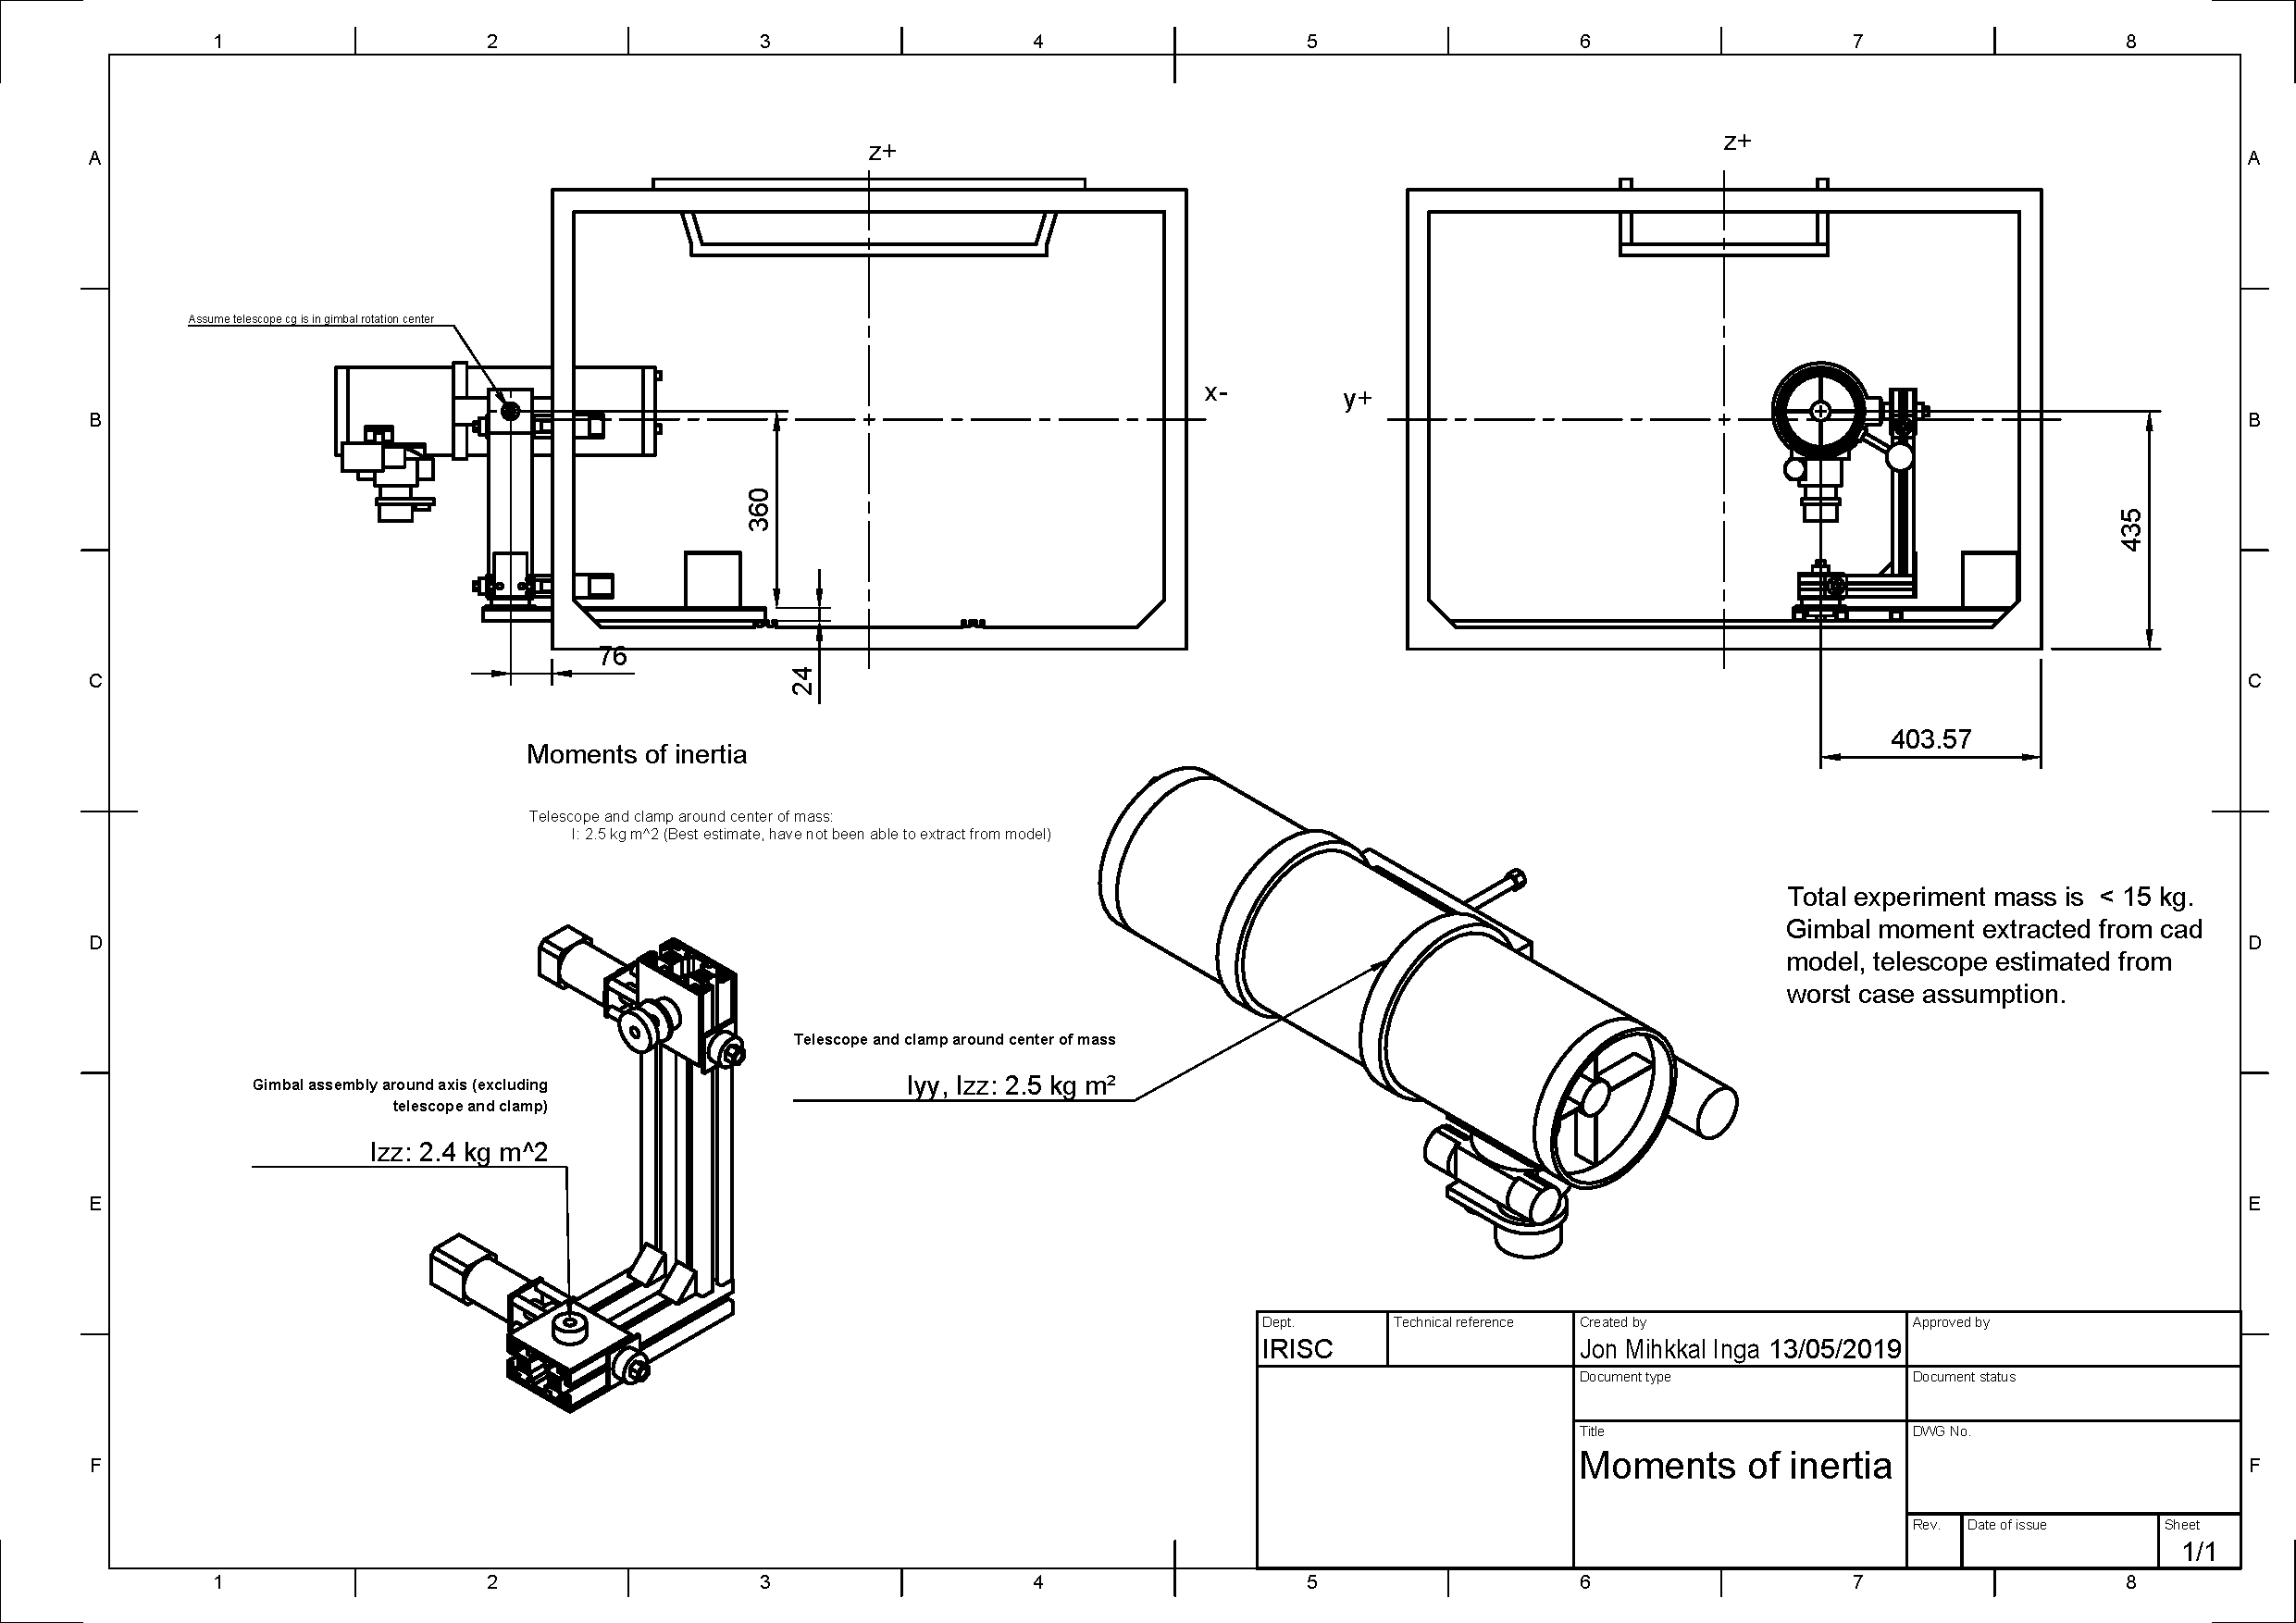
\includegraphics[scale=0.5]{appendix/img/mechanical_sketches/Moments.pdf}

\end{landscape}
\newpage
% \includepdf[scale=1,pages={1,2,3,4,5,6,7,8,9,10,11,12,13,14,15,16,17,18,19,20,21,22,23,24,25,26,27,28,29,30,31,32,33,34,35,36}]{appendix/pdf/manufacturing-drafts.pdf}


